%!TEX TS-program = xelatex

\documentclass[]{friggeri-cv}
\usepackage{ctex}
\usepackage{afterpage}
\usepackage{hyperref}
\hypersetup{
    pdftitle={devops-xidian},
    pdfauthor={PengFeng},
    pdfsubject={sub}
}
\usepackage{color}
\usepackage{xcolor}
\hypersetup{
    pdftitle={},
    pdfauthor={Feng},
    pdfsubject={},
    pdfkeywords={resume},
    colorlinks=false,       % no lik border color
   allbordercolors=white    % white border color for all
}
\addbibresource{bibliography.bib}
\RequirePackage{xcolor}
\definecolor{pblue}{HTML}{0395DE}
%header
\begin{document}
\header{恒生子}{校招}
      { 彭峰 } 
% 注意简历的下载位置更改和header的更改      
 %对应cls中的  node的三个   

% Fake text to add separator      
\fcolorbox{white}{gray}{\parbox{\dimexpr\textwidth-2\fboxsep-2\fboxrule}{%
.....
}}


\begin{aside}
  \section{工作意向}
    数据库工程师
%    运维工程师
%   系统工程师
%     技术运营
%    技术支持
%     系统运维工程师
%    Linux SA
%    运维开发攻城师
    ~
  \section{Phone \& Skype}
    17091314725
    18700833902
    ms6577
    ~
  \section{Email}
    \href{mailto:git4xuan@gmail.com}{\textbf{git4xuan@}\\gmail.com}
    \href{mailto:jobs@fengidea.com}{\textbf{jobs@}\\fengidea.com}
    ~
%  \section{在线简历}
%    \href{http://devops.mxuan.me}{devops.mxuan.me}
%    \href{https://bitbucket.org/neoben}{bitbucket.org/neoben}
%    \href{https://github.com/neoben}{github.com/neoben}
    ~
  \section{Programming}
  ~
    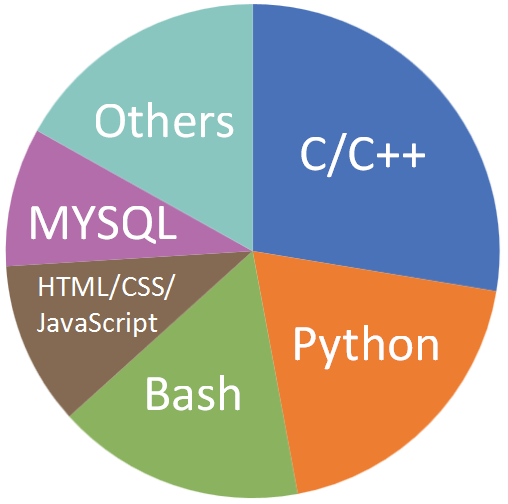
\includegraphics[scale=0.25]{img/programming3.png}
    ~
  \section{OS Preference}
  ~
    \textbf{openSUSE}
\includegraphics[scale=0.40]{img/5stars.png}
    \textbf{Debian}
\includegraphics[scale=0.40]{img/4stars.png}
    \textbf{CentOS}
\includegraphics[scale=0.40]{img/3stars.png}
    \textbf{Windows}
\includegraphics[scale=0.40]{img/3stars.png}
  ~
  \section{Personal Skills}
  ~
  \textbf{TCP/IP}
\includegraphics[scale=0.40]{img/4stars.png}
  \textbf{Nginx}
\includegraphics[scale=0.40]{img/4stars.png}
  \textbf{Vim}
\includegraphics[scale=0.40]{img/3stars.png}
  \textbf{Docker}
\includegraphics[scale=0.40]{img/2stars.png}
  \textbf{KVM}
\includegraphics[scale=0.40]{img/2stars.png}
  \textbf{Zabbix}
\includegraphics[scale=0.40]{img/2stars.png}
  \textbf{Puppet}
\includegraphics[scale=0.40]{img/1stars.png}
  \textbf{AWS}
\includegraphics[scale=0.40]{img/1stars.png}
  ~
\end{aside}

\section{项目介绍}
\begin{entrylist}
  \entry
    {02/15 - 08/15 }
    {虚拟化技术与平台}
    {Virtualization}
    {基于openSUSE 13.2的KVM,进行Vmware的P2V和到KVM下V2V的迁移。逻辑上简单参照Openstack,在硬盘上划分分区作为块分区的存储池,制作自用镜像。构建内网桥接环境和外网NAT环境。补充virt-manager中没有图形化实现的部分功能,编写CLI,在virsh和xml配置的基础上制定特定的虚拟机资源类型模板等,从而快速根据自身需要创建和使用干净的测试和学习环境。
    \\}   

   \entry
   {10/13 - 01/14}
   {基于树莓派的移动摄影车}
   {RaspberryPi}
   {
    树莓派在教育和ARM方面取得巨大的影响。项目中小车由Android客户端进行控制,Python调用GPIO接口利用L298N驱动板控制小车运动方向,使用USB接口的网络摄像头采集图像,在局域网下,以Web方式作为图像和视频的显示方式。\\
    个人负责任务协调,硬件设计和组装,以及Web界面。
   }
   
\end{entrylist}

\section{技能实践}
\begin{entrylist}
  \entry
    {12/15 - 02/16}
    {嵌入式显微成像系统}
    {Django}
    {在树莓派的基础上搭建的系统平台,在嵌入式系统下对光学薄膜进行数字显微成像和基本的图像处理,并可以远程显示和控制。内核进行系统配置实现集成化。硬件部分包括了光学衔接系统、显微采集硬件模块、光源设计等;Web界面实现图片显示与管理、基本图像处理等功能。\\
    整体使用B/S架构,Server端使用七牛API,并利用Docker进行部署。
   \\ }%考虑自己如何自己进行扩展,以及细节部分
  
  
  \entry
    {03/14 - 07/14 }
    {文件存储与共享}
    {Storage}
    {提供家庭一站式文件存储与共享功能,系统基于openSUSE,在局域网内利用KVM虚拟化提供SAMBA、NFS共享、FTP、DLNA、LEMP基础上搭建owncloud个人云等服务。\\}
    



\end{entrylist}

\section{校内经历}
\begin{entrylist}
  \entry
    {07/13 - 04/14}
    {校科协信息化实验室管理员}
    {Service \& Support}
    {\emph{服务器搭建与管理}
    适逢实验室添加新设备,负责计算机和交换机上报选型,为校科协多个部门提供技术支持和服务。包括:使用WindowsServer2008 R2实现路由和远程桌面服务,提供局域网内公共FTP和部门FTP文件共享,提供常见软件的安装和使用,部分Adobe系列软件培训,解决基本的网络问题。较好的实现了第一年实验室的技术支撑。  \\     
    }
    
\end{entrylist}


\newpage


\begin{aside}
~
~
  \section{Languages}
    \textbf{English}
\includegraphics[scale=0.40]{img/3stars.png}
  ~    
  \section{Self-Scoring}
    ~
    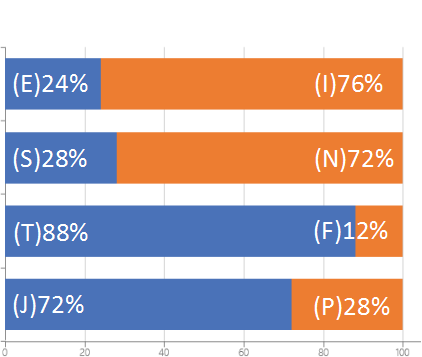
\includegraphics[scale=0.32]{img/personal.png}
    ~
  \section{Download Links}
    ~
    {\href{http://fengidea.qiniudn.com/ops-pengfeng-xidian.zip}{ZIP\_DOWNLOAD}}
   ~
%    {\href{http://fengidea.qiniudn.com/feng-read-xidian-1.pdf}{Book\_Read\_Part\_1.pdf}}
%    {\href{http://fengidea.qiniudn.com/feng-read-xidian-2.pdf}{Book\_Read\_Part\_2.pdf}}
%    {\href{http://fengidea.qiniudn.com/feng-read-xidian-3.jpg?imageView2/2/w/2560}{Book\_Read\_Part\_3.jpg}}
\end{aside}




\section{教育背景}
08/12\hspace{1mm}-\hspace{1mm}至今 \hspace{30mm} 电子科学与技术 \hspace{7mm}  西安电子科技大学  \hspace{7mm}  本科 \\

相关课程与内容:数字电路,微机原理与系统,电子元器件,光纤通信与应用,计算机图形学。\\


\section{其他信息}
%在这几年的学习中,我关注知识之间的联系性,注重知识的迁移。我更习惯先了解全局,在做出自己的决定。\\
%{简历下载链接:\href{http://fengidea.qiniudn.com/系统运维工程师-西电-58-彭峰.pdf}{系统运维工程师-西电-58-彭峰.pdf}}\\
%{图书馆部分阅读历史\_1(2015.07-2014.12):\href{http://fengidea.qiniudn.com/feng-read-xidian-1.pdf}{图书馆阅读历史-1}}\\
%{图书馆部分阅读历史\_2(2014.09-2012.10):\href{http://fengidea.qiniudn.com/feng-read-xidian-2.pdf}{图书馆阅读历史-2}}\\
%{部分购买书籍(截至2014.10):\href{http://fengidea.qiniudn.com/feng-read-xidian-3.pdf}{系统运维工程师-西电-58-彭峰.pdf}}
相比于侧重语言的细节,我更关注知识之间的联系、维系和概念迁移,全局意识较强。
这是一张自己整体知识的简单的知识点联系图:\\
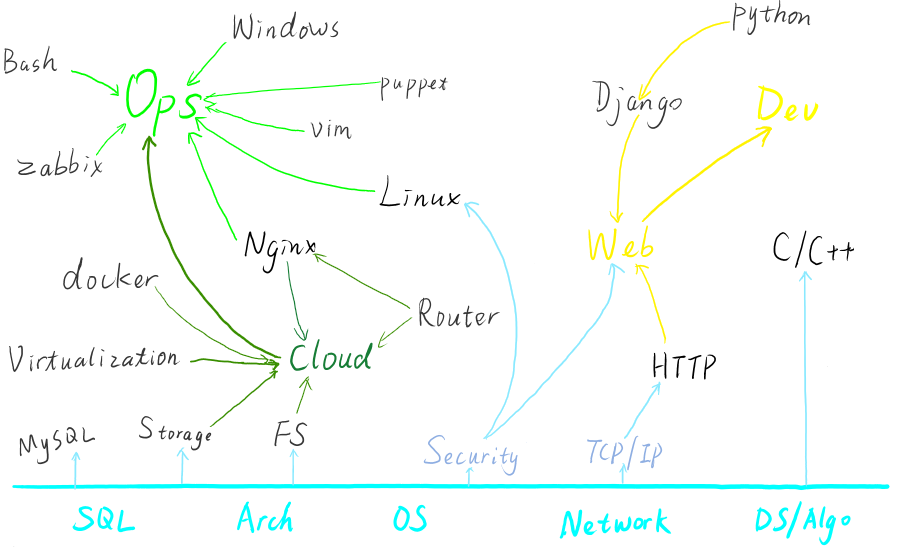
\includegraphics[scale=0.60]{img/devopsgraph.png}
Other Notes:部分借阅历史遗失(2014/09-2014/12);图片拍摄日期截至2014/12;旧博客弃用,开设时间请Whois;Github仅作为个人网盘和同步盘使用;Self-Scoring\hspace{1mm}基于MBTI(Step2);简历还在更新阶段。\\

\emph{如果您觉得我能很好的匹配到职位需求的话,还请不吝于联系我!此外,从性格上说我能接受各式的建议和反馈,其有助于自我改进和Review。本学校也有不少在贵公司就职的同学。\\
最后,非常感谢您花时间来阅读这份简历!\\}
~
\begin{flushleft}
\emph{3/1/2016}
\end{flushleft}
\begin{flushright}
\emph{彭峰}
\end{flushright}


\end{document}
